\chapter{Background}\label{ch:background}


\section{Cryptography Primitives}\label{sec:cryptography}

\subsection{Hash Functions}\label{subsec:crypto:hash}

Hash functions are cryptographic functions designed to behave like random
functions~\cite{smart2016randomOracleModel}.
When building a security proof, they can be assumed to have the following properties~\cite{smart2016randomOracleModel,
    smart2016hashFunctions}:
% FIXME needs references
\begin{description}
    \item[Determinism] A hash function always produces the same output for the same input
    \item[One-way] It is computationally impossible to compute the preimage for some output of a hash function
    \item[Uniformity] Outputs of a hash function are expected to be uniformly distributed.
    In practice, the output space of a hash function is finite, so \textit{collisions} (where two inputs produce the
    same output) are possible, but uniformity ensures this is an unlikely scenario.
\end{description}

\subsection{Symmetric key cryptography}

% TODO will i need this

\subsection{Public Key Cryptography}\label{subsec:crypto:pubkey}

In public key cryptography, two communicating parties (say Alice and Bob) can communicate privately by using pairs of
numbers that are related mathematically and which allow converting cleartext into cyphertext and
back~\cite{smart2016publicKey}.
This pair of numbers is called an asymmetric keypair, and is composed of a \textbf{public key} $e$ and a \textbf{private
key} $d$.\\

In this example, if Alice wishes to communicate with Bob, Bob can generate a keypair $(d, e)$ and publish $e$.
Alice can then encrypt her cleartext with $e$, and only Bob will be able to decrypt it (because only Bob knows $d$).

\begin{figure}[th]
    \centering
    \tikzset{every picture/.style={line width=0.75pt}} %set default line width to 0.75pt
    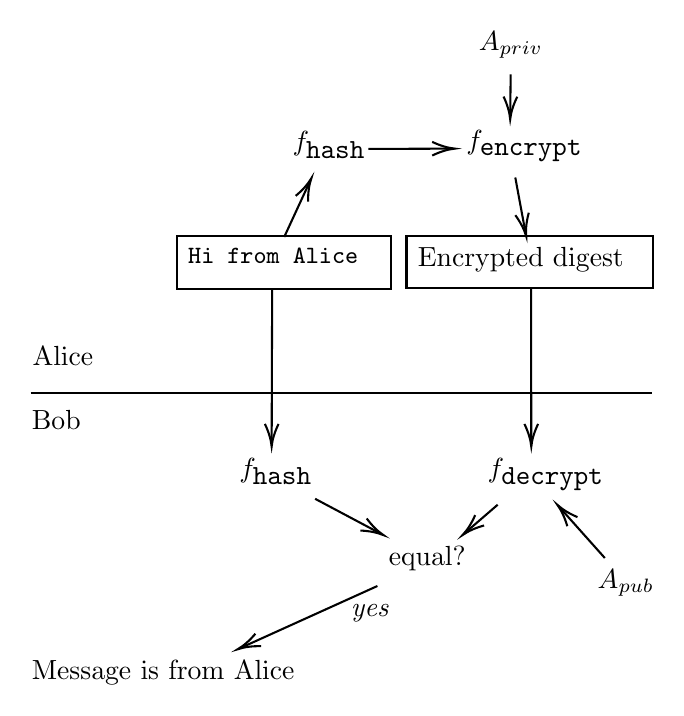
\begin{tikzpicture}[x=0.75pt,y=0.75pt,yscale=-1,xscale=1]
%uncomment if require: \path (0,355); %set diagram left start at 0, and has height of 355

%Straight Lines [id:da017592532205451983]
        \draw    (60.54,179.69) -- (359.87,179.69) ;

% Text Node
        \draw    (131,104) -- (234,104) -- (234,129.67) -- (131,129.67) -- cycle ;
        \draw (135,108.67) node [anchor=north west][inner sep=0.75pt]   [align=left] {\small \texttt{Hi from Alice}};
% Text Node
        \draw (185.33,52.33) node [anchor=north west][inner sep=0.75pt]   [align=left] {$\displaystyle f_{\texttt{hash}}$};
% Text Node
        \draw (275,4.33) node [anchor=north west][inner sep=0.75pt]   [align=left] {$\displaystyle A_{priv}$};
% Text Node
        \draw (332.33,263.33) node [anchor=north west][inner sep=0.75pt]   [align=left] {$\displaystyle A_{pub}$};
% Text Node
        \draw (269,52) node [anchor=north west][inner sep=0.75pt]   [align=left] {$\displaystyle f_{\texttt{encrypt}}$};
% Text Node
        \draw    (241.67,104) -- (360.67,104) -- (360.67,129.33) -- (241.67,129.33) -- cycle ;
        \draw (245.67,108.33) node [anchor=north west][inner sep=0.75pt]   [align=left] {Encrypted digest};
% Text Node
        \draw (60,156) node [anchor=north west][inner sep=0.75pt]   [align=left] {Alice};
% Text Node
        \draw (59.67,186.67) node [anchor=north west][inner sep=0.75pt]   [align=left] {Bob};
% Text Node
        \draw (159.67,209.67) node [anchor=north west][inner sep=0.75pt]   [align=left] {$\displaystyle f_{\texttt{hash}}$};
% Text Node
        \draw (279.33,209.67) node [anchor=north west][inner sep=0.75pt]   [align=left] {$\displaystyle f_{\texttt{decrypt}}$};
% Text Node
        \draw (231.67,252.33) node [anchor=north west][inner sep=0.75pt]   [align=left] {equal?};
% Text Node
        \draw (59.67,307.33) node [anchor=north west][inner sep=0.75pt]   [align=left] {Message is from Alice};
% Text Node
        \draw (208.67,280.33) node [anchor=north west][inner sep=0.75pt]   [align=left] {\textit{{ yes}}};
% Connection
        \draw    (182.78,104.67) -- (195.03,78.15) ;
        \draw [shift={(195.87,76.33)}, rotate = 114.8] [color={rgb, 255:red, 0; green, 0; blue, 0 }  ][line width=0.75]    (10.93,-3.29) .. controls (6.95,-1.4) and (3.31,-0.3) .. (0,0) .. controls (3.31,0.3) and (6.95,1.4) .. (10.93,3.29)   ;
% Connection
        \draw    (223.33,62.25) -- (263,62.11) ;
        \draw [shift={(265,62.1)}, rotate = 179.79] [color={rgb, 255:red, 0; green, 0; blue, 0 }  ][line width=0.75]    (10.93,-3.29) .. controls (6.95,-1.4) and (3.31,-0.3) .. (0,0) .. controls (3.31,0.3) and (6.95,1.4) .. (10.93,3.29)   ;
% Connection
        \draw    (294.1,76) -- (298.98,102.37) ;
        \draw [shift={(299.35,104.33)}, rotate = 259.5] [color={rgb, 255:red, 0; green, 0; blue, 0 }  ][line width=0.75]    (10.93,-3.29) .. controls (6.95,-1.4) and (3.31,-0.3) .. (0,0) .. controls (3.31,0.3) and (6.95,1.4) .. (10.93,3.29)   ;
% Connection
        \draw    (291.87,26.33) -- (291.66,46) ;
        \draw [shift={(291.64,48)}, rotate = 270.59] [color={rgb, 255:red, 0; green, 0; blue, 0 }  ][line width=0.75]    (10.93,-3.29) .. controls (6.95,-1.4) and (3.31,-0.3) .. (0,0) .. controls (3.31,0.3) and (6.95,1.4) .. (10.93,3.29)   ;
% Connection
        \draw    (176.96,129.67) -- (176.72,203.67) ;
        \draw [shift={(176.71,205.67)}, rotate = 270.19] [color={rgb, 255:red, 0; green, 0; blue, 0 }  ][line width=0.75]    (10.93,-3.29) .. controls (6.95,-1.4) and (3.31,-0.3) .. (0,0) .. controls (3.31,0.3) and (6.95,1.4) .. (10.93,3.29)   ;
% Connection
        \draw    (301.69,129.33) -- (301.81,203.67) ;
        \draw [shift={(301.81,205.67)}, rotate = 269.91] [color={rgb, 255:red, 0; green, 0; blue, 0 }  ][line width=0.75]    (10.93,-3.29) .. controls (6.95,-1.4) and (3.31,-0.3) .. (0,0) .. controls (3.31,0.3) and (6.95,1.4) .. (10.93,3.29)   ;
% Connection
        \draw    (197.67,230.82) -- (228.87,247.4) ;
        \draw [shift={(230.63,248.33)}, rotate = 207.98] [color={rgb, 255:red, 0; green, 0; blue, 0 }  ][line width=0.75]    (10.93,-3.29) .. controls (6.95,-1.4) and (3.31,-0.3) .. (0,0) .. controls (3.31,0.3) and (6.95,1.4) .. (10.93,3.29)   ;
% Connection
        \draw    (285.62,233.67) -- (270.15,247.03) ;
        \draw [shift={(268.64,248.33)}, rotate = 319.18] [color={rgb, 255:red, 0; green, 0; blue, 0 }  ][line width=0.75]    (10.93,-3.29) .. controls (6.95,-1.4) and (3.31,-0.3) .. (0,0) .. controls (3.31,0.3) and (6.95,1.4) .. (10.93,3.29)   ;
% Connection
        \draw    (227.67,272.83) -- (162.1,302.51) ;
        \draw [shift={(160.28,303.33)}, rotate = 335.64] [color={rgb, 255:red, 0; green, 0; blue, 0 }  ][line width=0.75]    (10.93,-3.29) .. controls (6.95,-1.4) and (3.31,-0.3) .. (0,0) .. controls (3.31,0.3) and (6.95,1.4) .. (10.93,3.29)   ;
% Connection
        \draw    (337.23,259.33) -- (315.66,235.16) ;
        \draw [shift={(314.33,233.67)}, rotate = 48.25] [color={rgb, 255:red, 0; green, 0; blue, 0 }  ][line width=0.75]    (10.93,-3.29) .. controls (6.95,-1.4) and (3.31,-0.3) .. (0,0) .. controls (3.31,0.3) and (6.95,1.4) .. (10.93,3.29)   ;

    \end{tikzpicture}
    \decoRule
    \caption[Asymmetric signing scheme]{An asymmetric key signing scheme where Bob is able to verify only Alice could
    have written '\texttt{Hi from Alice}'}
    \label{fig:pubkey-signing}
\end{figure}

Conversely, the same keypair can be used by Bob to send a message to Alice where Alice can verify that only Bob
could have written the message.
This is called \textit{signing}~\cite{smart2016signatures} and, more generally, it allows a sender of a message to
prove they are the authors of the message to a recipient.
An example of a signing scheme can be seen in Figure~\ref{fig:pubkey-signing}.

\subsection{Secure Digital Timestamps}\label{subsec:crypto:timestamps}
% TODO citation for definiton
\textit{Trusted (digital) timestamping} is the process of securely proving that a document (for our purposes, a blob of
bytes) was created, was modified at, or existed at a certain point in time.
% TODO citation for widely used
In industry this is commonly implemented by trusting a Time Stamping Authority (TSA)~\cite{timestamps_tsp_rfc} that
signs (see~\nameref{subsec:crypto:pubkey}) a concatenation of the hash of the document and a timestamp representing some
time $t$.
Therefore a party that trusts the TSA to provide the right timestamp can verify that, when the TSA made the signature,
the current time was $t$.
\\

This method can be used for confidential data because the TSA does not perform the hashing of the original document
themselves - they are exposed only to its digest.

Additionally, the requester of the timestamp cannot deny they were not in possession of the original data at the time
% TODO verify statement
$t$ given by the timestamp, because it was them that produced its hash digest.

\subsubsection{Decentralised Timestamps}

Secure timestamps can also be achieved without relying on trusted parties by publishing the document digest to a
blockchain~\cite{gipp2015timestamps_btc}: blocks are public and cannot be tampered with (see~\nameref{subsec:btc:pow}),
so putting a signed digest in a block shows that the signer knew the original document at the time the block was
accepted by the network.


\section{Bitcoin Protocol}\label{sec:bitcoin}

Blockchain technology was introduced by~\cite{nakamoto2008bitcoin} as a decentralised system allowing for electronic
cash payments.
Blockchains are immutable distributed ledgers where participants' balances can be verified by every other participant,
and it is computationally hard to tamper with balances to perform attacks (such as performing a transaction where a
participant spends more funds than what they own). \\
I will provide a brief overview of how Bitcoin provides these guarantees.

\subsection{Transactions}\label{subsec:btc:txs}

\cite{nakamoto2008bitcoin} defines an \textit{electronic coin} as a chain of signatures: a payer can use their private
key, the hash of the previous transaction, and the payee's public key to create a signed hash that can be verified by
the payee (and used by them for \textit{their} next transaction).
This is illustrated in Figure~\ref{fig:bitcoin-tx}.

\begin{figure}[th]
    \centering
    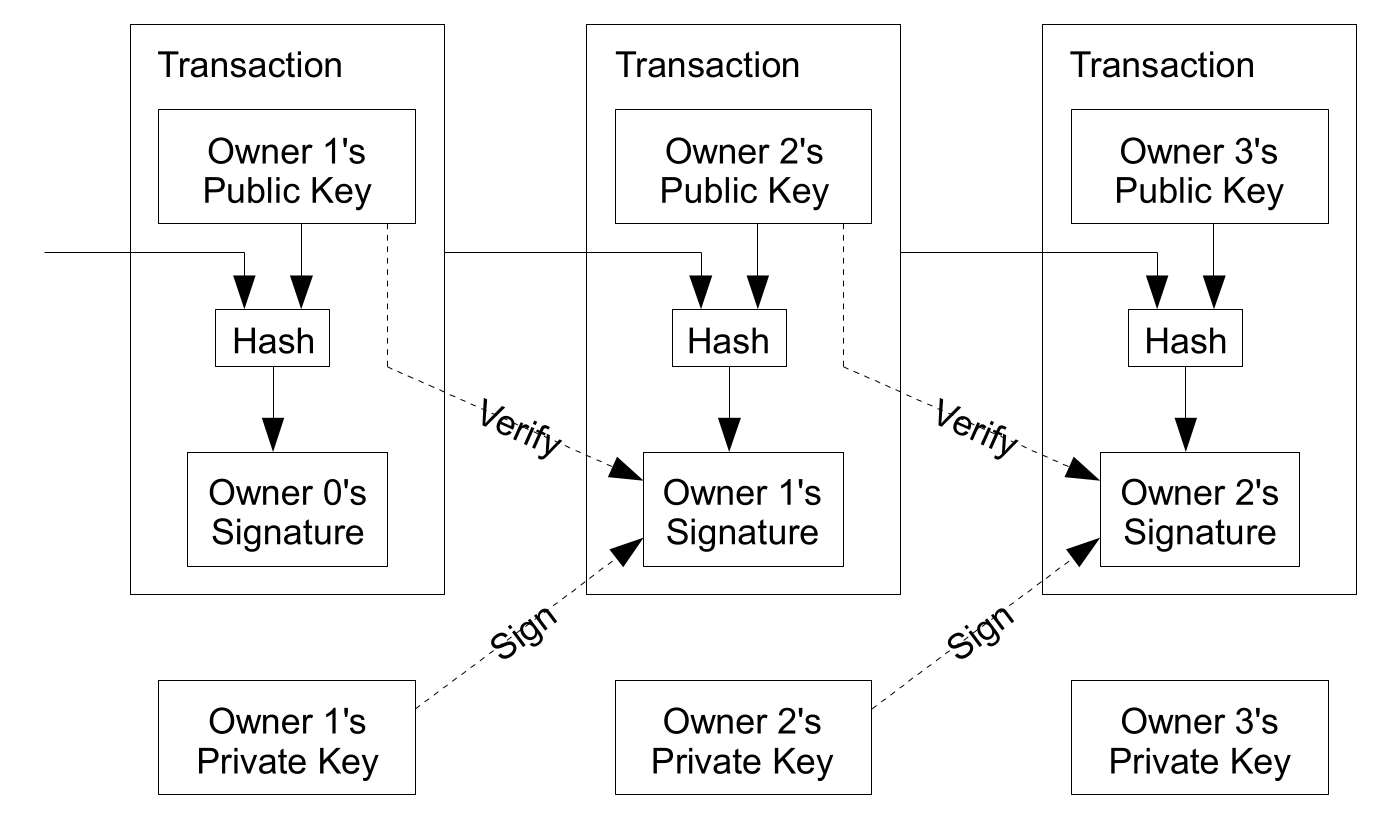
\includegraphics[width=0.8\columnwidth]{figures/bitcoin-tx}
    \caption[Bitcoin coin ownership transfer]{Transfer of ownership signature chain, from~\cite{nakamoto2008bitcoin}}
    \label{fig:bitcoin-tx}
\end{figure}

This ensures that, as long as a participants sign transactions at most once:
\begin{itemize}
    \item By verifying the chain of signatures, every participant can verify which participant owns which coin
    \item Only the owner of a coin can initiate a transaction with that coin
\end{itemize}

Bitcoin enforces that participants can only sign transactions once thanks to its proof-of-work
(see~\ref{subsec:btc:pow}) algorithm.

\subsection{Proof-Of-Work}\label{subsec:btc:pow}

Bitcoin ensures 'unique signatures' in transactions by grouping transactions in immutable, public \textit{blocks}.
Participants can then verify a payer has not signed a hash of a single transaction twice by looking at all existing
transactions.\\

Blocks are made immutable by including in them a value (called a \textit{nonce}) and the hash of the previous block.
% TODO verify it is the hash of the entire block that must yield the zeroes (implementation detail really)
The protocol then accepts only blocks where the $n$ first bits of its hash are zeroes. \\

Thus, in order to publish a block a participant must do work to find a nonce such that the block's hash meets this
condition - then other participants can verify its validity with a single hash operation.
This guarantees that a block cannot be changed (ie, a new copy published) without redoing the computational work.
Because blocks are chained (they include the hash of the previous block), in order to modify a transaction in the past
an adversary needs to redo the computational work for every block since that transaction (see Figure
\ref{fig:bitcoin-blockchain}).
% TODO implementation of mining rewards
Additionally, participants that successfully find a suitable nonce and propose new blocks (also referred to as
\textit{miners}) are allowed to add a specific transaction to the block where they own a newly created coin (also
referred to as \textit{mining reward}).

\begin{figure}[th]
    \centering
    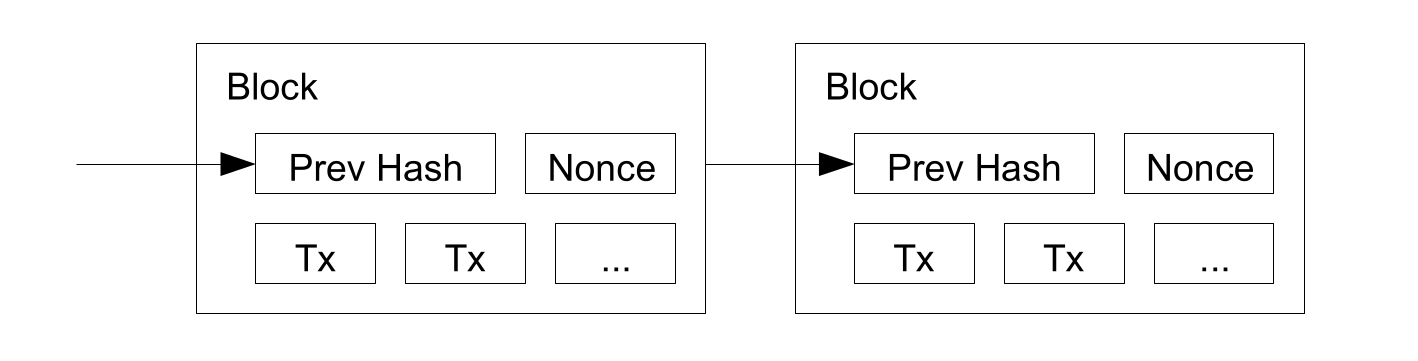
\includegraphics[width=0.8\columnwidth]{figures/bitcoin-blockchain}
    \caption[Two last blocks in a blockhain]{Two last blocks in a blockchain, from~\cite{nakamoto2008bitcoin}}
    \label{fig:bitcoin-blockchain}
\end{figure}


This model of consensus ensures that
\begin{itemize}
    \item Participants have a monetary incentive to stay honest with respect to the protocol
    \item An honest chain will out-compete an adversary's chain as long as the majority of computing power is honest
\end{itemize}

\subsection{Further details of the Bitcoin protocol}\label{subsec:btc.details}

While I provide a high-level overview of what makes the protocol function, there are many more details that combined
allow for more efficiency and usability:
\begin{itemize}
    \item Transactions may have several inputs and outputs, so participants can transfer amounts rather than single
    \textit{electronic coins}.
    Thus, a participant's balance is the sum of all the unspent outputs of previous transactions.
    \item By modifying how many of the leading bits of a blocks' hash must be zeroes, the average computation necessary
    to produce a new block can be adjusted by the protocol.
    \item By using Merkle Trees~\cite{merkle1980tree} transactions with fully spent transaction outputs can be discarded
    without breaking the block's hash.
    This allows compacting old blocks to reclaim disk space.
    \item A participant that does not wish to mine or hold a copy of the entire blockchain can still verify payments.
    It can keep a copy of the block headers of the longest chain and link a transaction to where it is on-chain and
    check that other network nodes have accepted it.
\end{itemize}
\\
For more information on all the workings of the Bitcoin protocol, please refer to~\cite{nakamoto2008bitcoin}.


\section{Ethereum Smart Contracts}\label{sec:ethereum}
% TODO idk to what extent I will need this?

Smart contracts were first formalised by~\cite{szabo1997smart-contracts} and implemented in~\cite{buterin2015ethereum}


\section{Zero-Knowledge Proofs}

An \textit{Interactive Proof} is a protocol where a verifier $V$ either \textit{accepts} or \textit{rejects} whether a
prover $P$ knows something~\cite{damgaard1998zk_protocols}.
For example, $P$ could be trying to convince $V$ that they know the preimage of a hash.

An interactive proof system has two key properties~\cite{smart2016zeroknowledgeproofs}:
\begin{description}
    \item[Completeness] If $P$ knows the thing being proved and follows the protocol, then $V$ should accept with
    probability one.
    \item[Soundness] If $P$ does not know the thing being proved, then $V$ should only have a negligible probability of
    accepting.
\end{description}

A \textit{Zero-Knowledge Proof} is an interactive proof with the additional property of \textit{zero-knowledge}, where
$V$ accepts without having learned any new information during their exchange with $P$~\cite{damgaard1998zk_protocols,
    smart2016zeroknowledgeproofs}.
In our example, a zero-knowledge proof where $P$ convinces $V$ that they know the preimage of a hash would require $P$
not sharing any information about (or related to) the preimage itself.

This protocol has the interesting property that the information $P$ has proven to know is still private to $V$, and
$V$ is unable to reproduce the proof and convince a third party (say, $V'$) that they (or $P$) know that information.

%  TODO maybe talk about assumptions like unbounded computation

\subsection{Zero-Knowledge Succinct Arguments of Knowledge (zk-SNARKs)}

Interactive proofs assume the prover is computationally unbounded (and so worries about computationally
unbounded adversaries), but by relaxing the soundness property to computationally sound proofs we can assume a
polynomial time prover~\cite{damgaard1998zk_protocols}.

This variation of an interactive proof is called an \textit{interactive argument} (because an unbounded adversary would be
able to fool $V$)~\cite{smart2016zeroknowledgeproofs}.

If we also preserve the zero-knowledge property, we have an \textit{zero-knowledge argument}, which can now be
efficient because it can run in polynomial time~\cite{naranker2022zeroknowledge}.

Additionally, if the prover is unable to construct a proof without some sort of secret (in our previous example, the
preimage of a hash function), then we have an argument \textit{of knowledge}.
Intuitively, in a zero-knowledge argument of knowledge, $V$ becomes convinced that $P$ knows some secret without the
protocol leaking any information about the secret.\\

If our zero-knowledge argument of knowledge additionally satisfies the properties of being \textit{non-interactive}~(no
or little interaction between prover and verifier) and \textit{succinct}~(the sizes of the messages are small in
comparison to the length of the actual computation), then we have a \textit{Zero-Knowledge Succinct Argument of
Knowledge} (or \textit{zk-SNARK})~\cite{reitwiessner2016zksnarks}.

Recent applications of zk-SNARKs include privacy preserving blockchains (see~\ref{sec:bitcoin}) where a network can
verify a participant does not spend more funds that their balance, without leaking any knowledge of the amount being
spent or the balance itself~\cite{zerocash_whitepaper}.

% TODO mention zksnarks in eth smart contracts? or maybe wait for it?


\section{Licensing}
% TODO

\subsection{Dataset Licesing}
% TODO
